\chapter{Introduction} 


\section{What is Machine Learning?}
\begin{itemize} 
    \item Arthur Samuel described it as: 
    ``the field of study that gives computers the ability to learn without being explicitly programmed.'' 
    This is an older, informal definition.
    \item Tom Mitchell provides a more modern definition: 
    ``A computer program is said to learn from experience E with respect to some class of tasks T and performance measure P, 
    if its performance at tasks in T, as measured by P, improves with experience E.'' 
\end{itemize}


\section{Supervised Learning}
\begin{itemize} 
    \item Given a data set and already know the correct output. 
    \item Are categorized into ``regression'' and ``classification'' problems. 
    \item In a regression problem, we are trying to predict results within a continuous output, meaning that we are trying to map input variables to some continuous function.
    \item In a classification problem, we are instead trying to predict results in a discrete output. In other words, we are trying to map input variables into discrete categories. 
\end{itemize}
\begin{figure}[!htbp]
    \begin{minipage}[t]{0.5\textwidth}
        \centering
        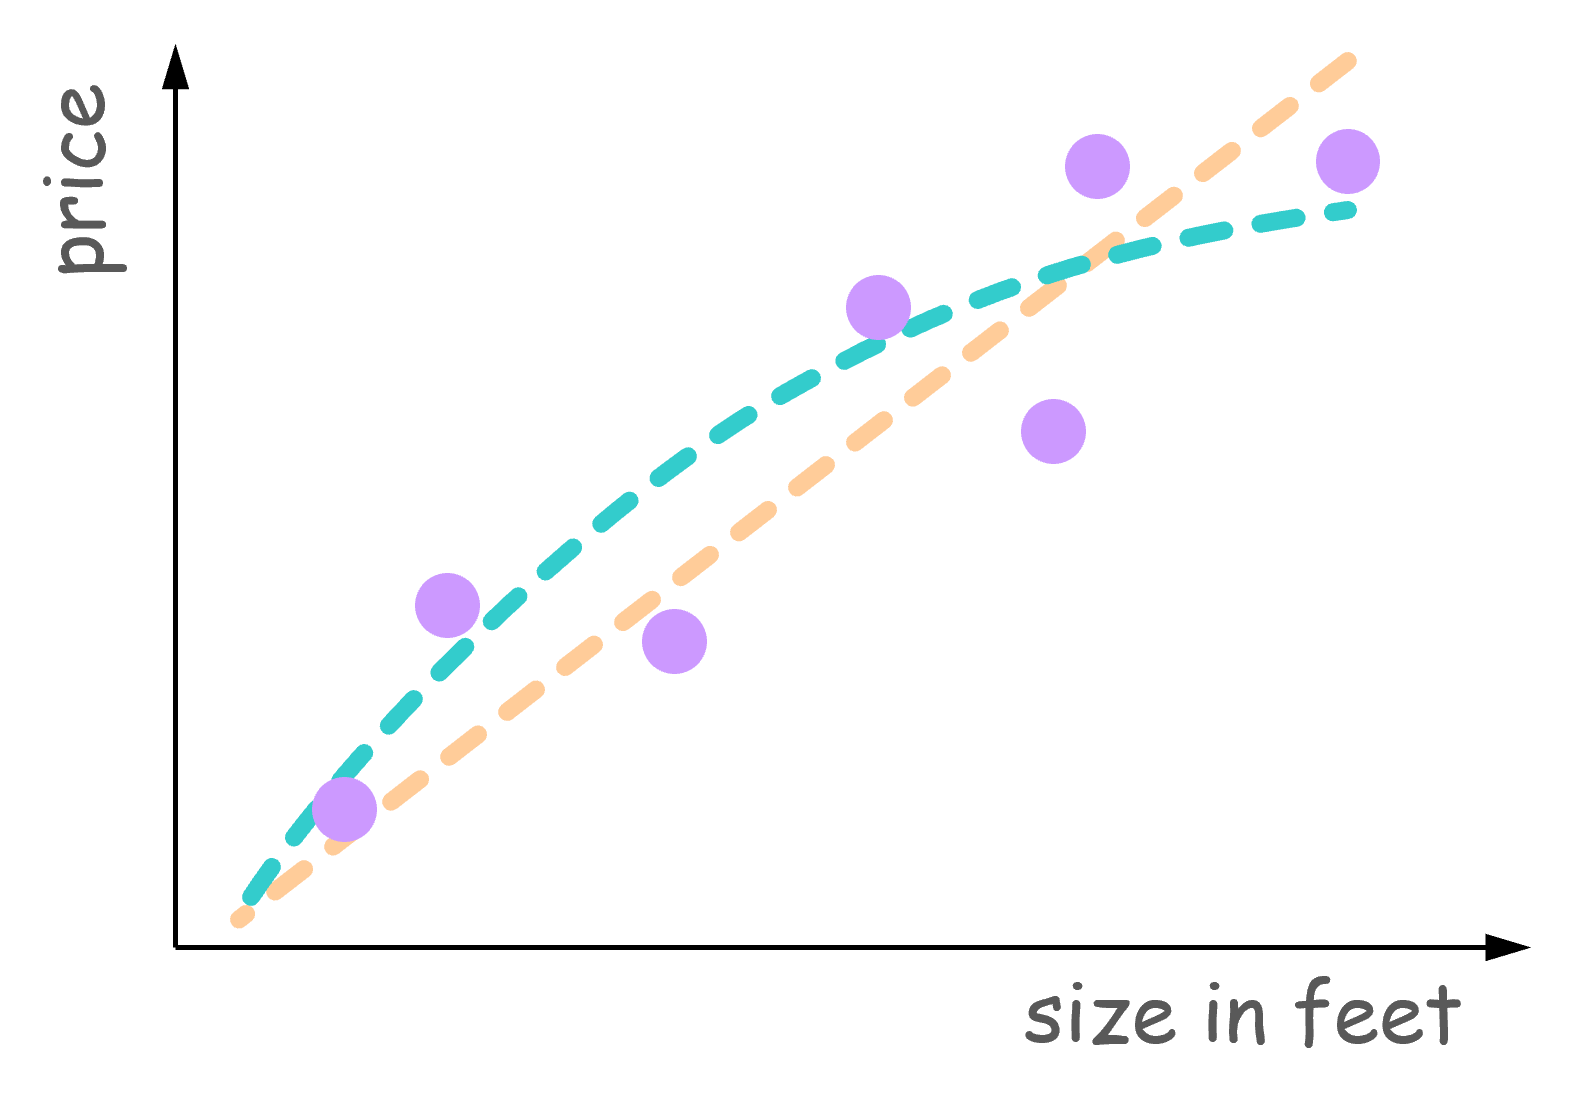
\includegraphics[width=2.4in]{./images/house_price.png}
        \caption{House price}
    \end{minipage}
    \begin{minipage}[t]{0.45\textwidth}
        \centering
        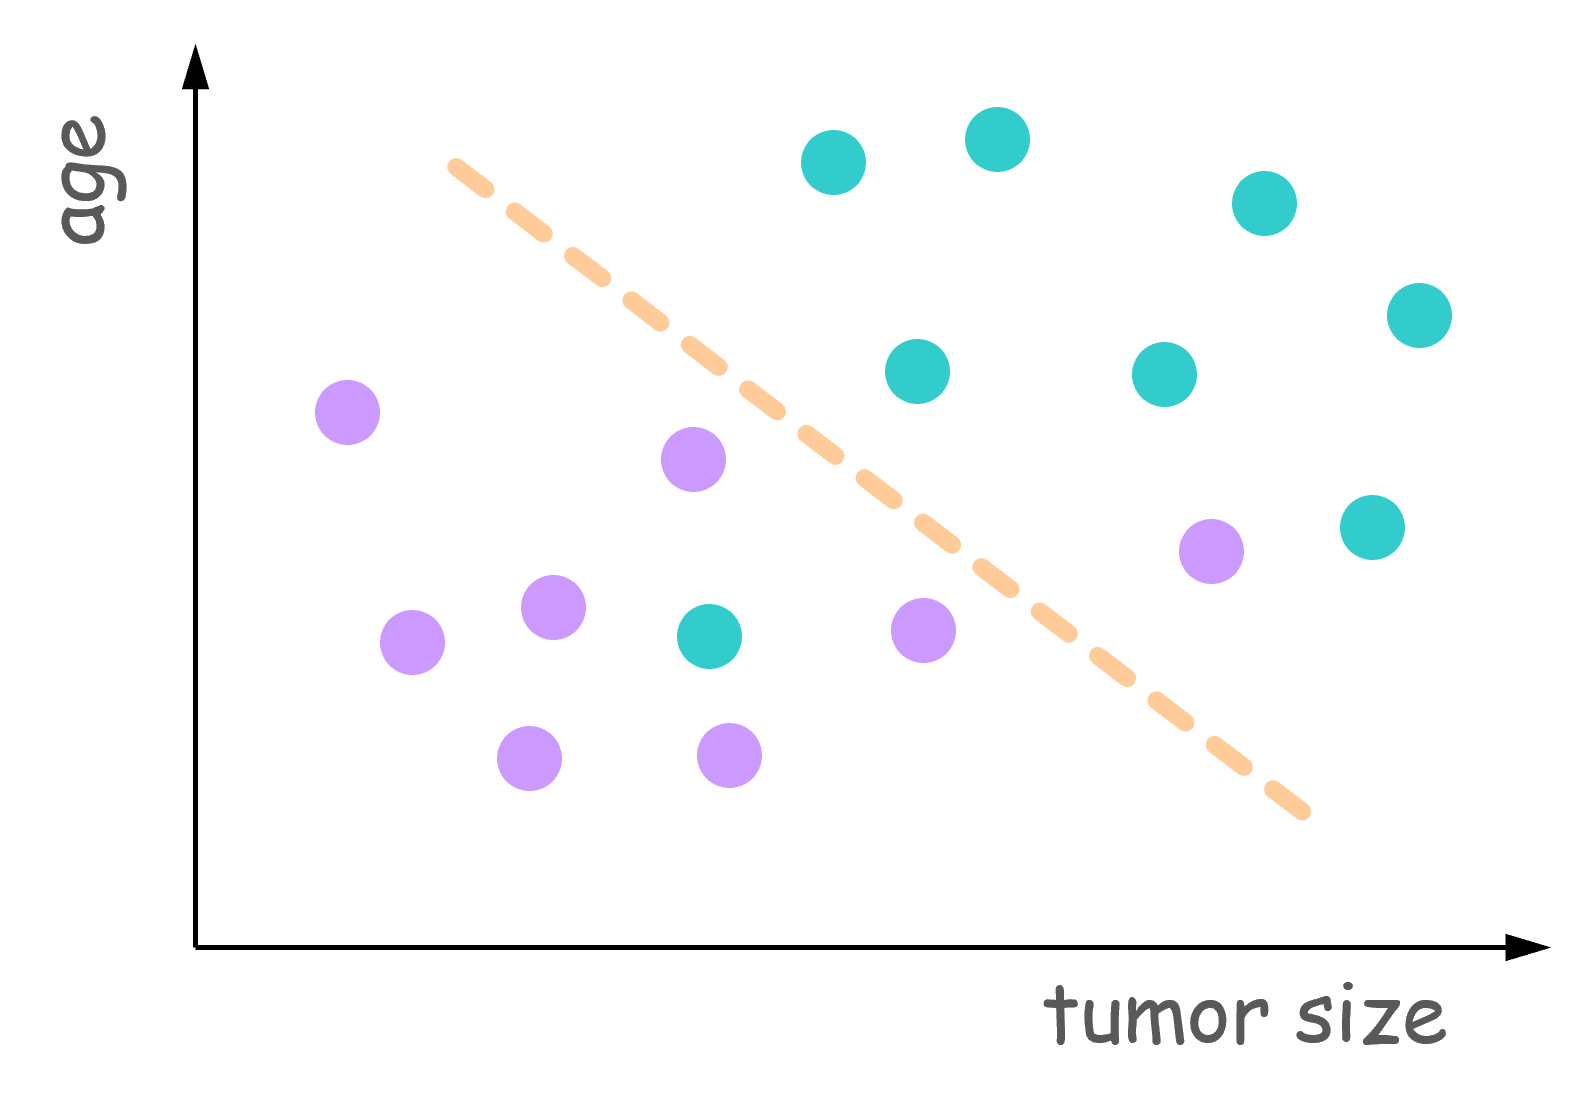
\includegraphics[width=2.4in]{./images/tumor_size.png}
        \caption{Tumor size}
    \end{minipage}
\end{figure}


\section{Unsupervised Learning}
\begin{itemize} 
    \item Approach problems with little or no idea what our results should look like. 
    \item We can derive this structure by clustering the data based on relationships among the variables in the data.
    \item There is no feedback based on the prediction results.
\end{itemize}
\begin{figure}[!htbp]
    \begin{minipage}[t]{0.5\textwidth}
        \centering
        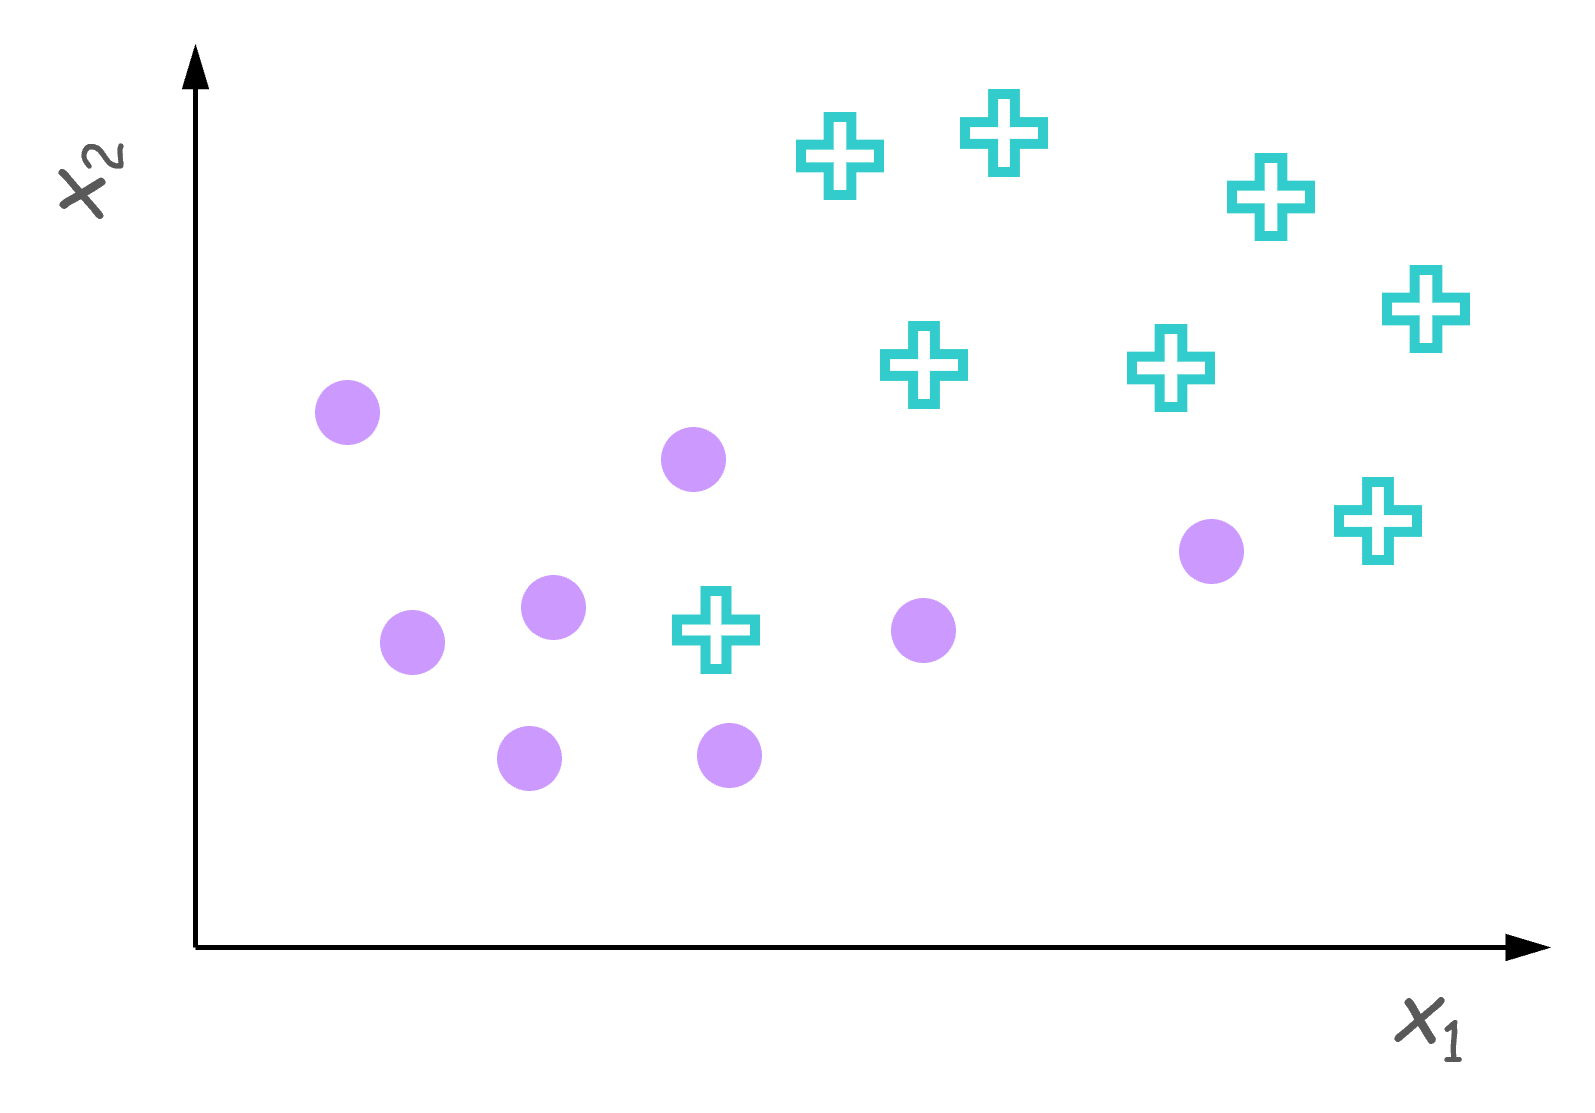
\includegraphics[width=2.0in]{./images/supervised.png}
        \caption{Supervised Learning}
    \end{minipage}
    \begin{minipage}[t]{0.45\textwidth}
        \centering
        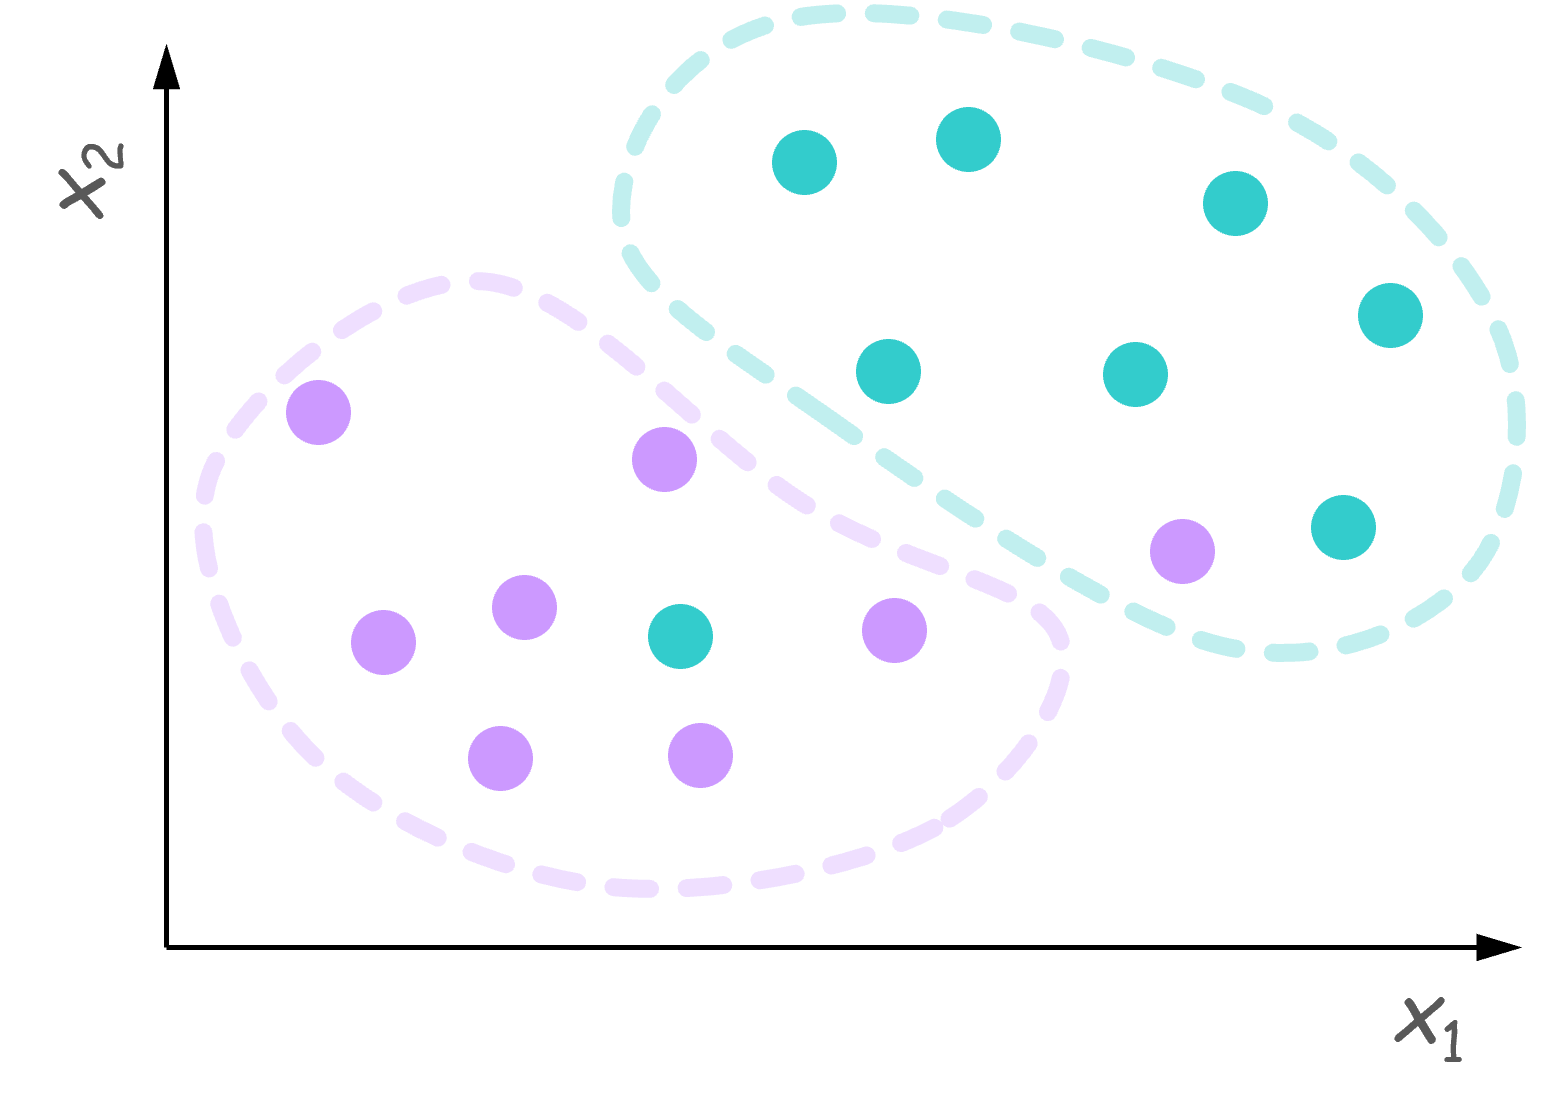
\includegraphics[width=2.0in]{./images/unsupervised.png}
        \caption{Unsupervised Learning}
    \end{minipage}
\end{figure}
